\documentclass[tikz, border=5pt]{standalone}

\usepackage{amsmath,amssymb}
\usepackage{xcolor}
\usetikzlibrary{arrows.meta, shadows.blur, shapes.geometric}

\definecolor{utnblue}{RGB}{0, 51, 102}

\begin{document}
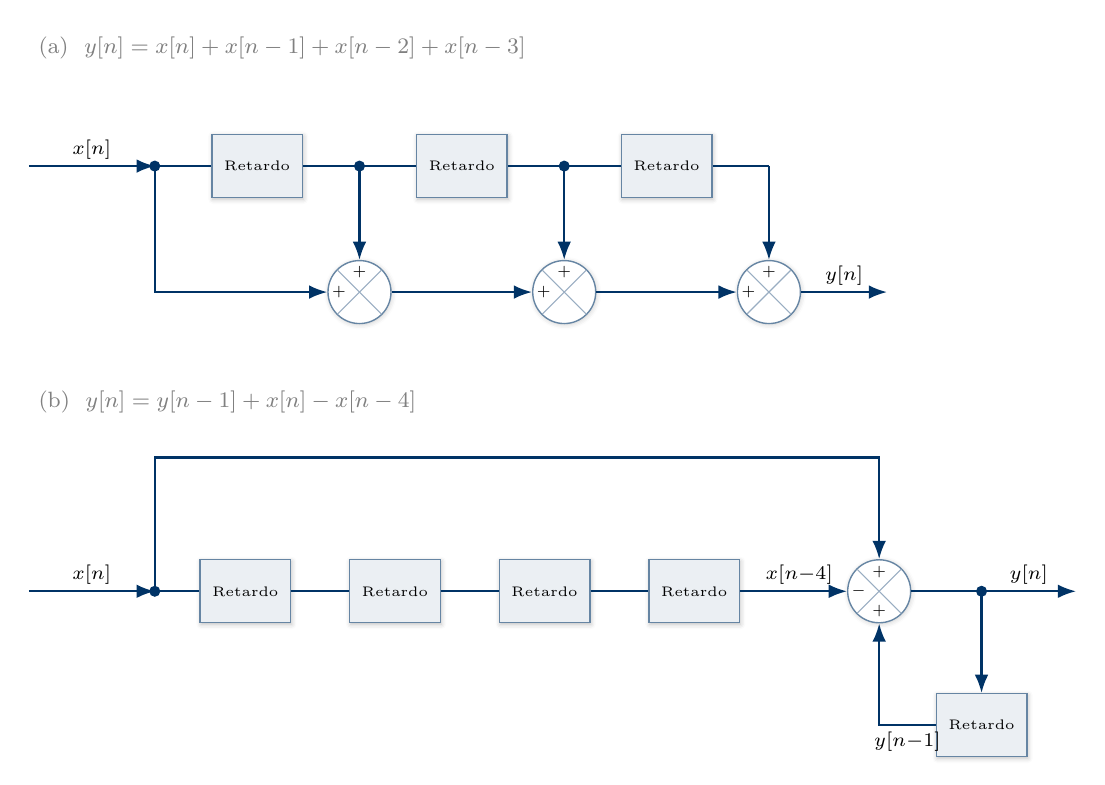
\begin{tikzpicture}[>=Latex, font=\small,
    delay/.style={
        draw=utnblue!60, line width=0.5pt, fill=utnblue!8,
        minimum width=1.15cm, minimum height=0.8cm, font=\tiny,
        blur shadow={shadow blur steps=4, shadow blur extra rounding=0pt,
                     shadow xshift=0.4pt, shadow yshift=-0.6pt, shadow opacity=25}
    },
    sum/.style={
        draw=utnblue!60, line width=0.5pt, circle, minimum size=0.8cm,
        inner sep=0pt, fill=white,
        blur shadow={shadow blur steps=4, shadow blur extra rounding=0pt,
                     shadow xshift=0.3pt, shadow yshift=-0.4pt, shadow opacity=20}
    },
    cross_line/.style={utnblue!40, line width=0.4pt},
    signal/.style={->, thick, utnblue},
    wire/.style={-, thick, utnblue},
    tlab/.style={font=\scriptsize, inner sep=2pt, text=black},
]

% ================= (a) forma no recursiva =================
\begin{scope}[shift={(0,0)}]
    \node[font=\footnotesize, gray, anchor=west] at (-1.6,1.5)
        {(a) \ $y[n]=x[n]+x[n-1]+x[n-2]+x[n-3]$};

    \coordinate (in) at (-1.6,0);
    \coordinate (p0) at (0,0);
    \node[delay] (D1) at (1.3,0) {Retardo};
    \coordinate (p1) at (2.6,0);
    \node[delay] (D2) at (3.9,0) {Retardo};
    \coordinate (p2) at (5.2,0);
    \node[delay] (D3) at (6.5,0) {Retardo};
    \coordinate (p3) at (7.8,0);

    \node[sum] (S1) at (2.6,-1.6) {};
    \node[sum] (S2) at (5.2,-1.6) {};
    \node[sum] (S3) at (7.8,-1.6) {};
    \foreach \s in {S1,S2,S3}{
        \draw[cross_line] ($(\s)+(-0.28,-0.28)$) -- ($(\s)+(0.28,0.28)$);
        \draw[cross_line] ($(\s)+(-0.28,0.28)$) -- ($(\s)+(0.28,-0.28)$);
        \node[font=\tiny] at ($(\s)+(-0.26,0)$) {$+$};
        \node[font=\tiny] at ($(\s)+(0,0.25)$) {$+$};
    }
    \coordinate (out) at (9.3,-1.6);

    \draw[signal] (in) -- (p0) node[tlab, above, midway] {$x[n]$};
    \draw[wire] (p0) -- (D1.west);
    \draw[wire] (D1.east) -- (p1);
    \draw[wire] (p1) -- (D2.west);
    \draw[wire] (D2.east) -- (p2);
    \draw[wire] (p2) -- (D3.west);
    \draw[wire] (D3.east) -- (p3);
    \foreach \p in {p0,p1,p2}{ \fill[utnblue] (\p) circle (2.0pt); }

    \draw[signal] (p0) |- (S1.west);
    \draw[signal] (p1) -- (S1.north);
    \draw[signal] (S1.east) -- (S2.west);
    \draw[signal] (p2) -- (S2.north);
    \draw[signal] (S2.east) -- (S3.west);
    \draw[signal] (p3) -- (S3.north);
    \draw[signal] (S3.east) -- (out) node[tlab, above, midway] {$y[n]$};
\end{scope}

% ================= (b) forma recursiva =================
\begin{scope}[shift={(0,-5.4)}]
    \node[font=\footnotesize, gray, anchor=west] at (-1.6,2.4)
        {(b) \ $y[n]=y[n-1]+x[n]-x[n-4]$};

    \coordinate (in) at (-1.6,0);
    \coordinate (q0) at (0,0);
    \node[delay] (E1) at (1.15,0) {Retardo};
    \node[delay] (E2) at (3.05,0) {Retardo};
    \node[delay] (E3) at (4.95,0) {Retardo};
    \node[delay] (E4) at (6.85,0) {Retardo};
    \coordinate (q4) at (8.0,0);

    \node[sum] (S) at (9.2,0) {};
    \draw[cross_line] ($(S)+(-0.28,-0.28)$) -- ($(S)+(0.28,0.28)$);
    \draw[cross_line] ($(S)+(-0.28,0.28)$) -- ($(S)+(0.28,-0.28)$);
    \node[font=\tiny] at ($(S)+(-0.26,0)$) {$-$};
    \node[font=\tiny] at ($(S)+(0,0.25)$) {$+$};
    \node[font=\tiny] at ($(S)+(0,-0.25)$) {$+$};

    \coordinate (tap) at (10.5,0);
    \coordinate (out) at (11.7,0);
    \node[delay] (E5) at (10.5,-1.7) {Retardo};

    \draw[signal] (in) -- (q0) node[tlab, above, midway] {$x[n]$};
    \fill[utnblue] (q0) circle (2.0pt);
    \draw[wire] (q0) -- (E1.west);
    \draw[wire] (E1.east) -- (E2.west);
    \draw[wire] (E2.east) -- (E3.west);
    \draw[wire] (E3.east) -- (E4.west);
    \draw[wire] (E4.east) -- (q4);
    \draw[signal] (q4) -- (S.west) node[tlab, above, midway, xshift=-6pt] {$x[n{-}4]$};

    \draw[signal] (q0) |- (9.2,1.7) -- (S.north);
    \draw[wire] (S.east) -- (tap);
    \fill[utnblue] (tap) circle (2.0pt);
    \draw[signal] (tap) -- (out) node[tlab, above, midway] {$y[n]$};
    \draw[signal] (tap) -- (E5.north);
    \draw[signal] (E5.west) -| (S.south) node[tlab, below, pos=0.25] {$y[n{-}1]$};
\end{scope}

\end{tikzpicture}
\end{document}
